\documentclass[spanish]{mathnotes}

% Title page
\title{Métodos numéricos para EDP}
\subtitle{Estimación de error a posteriori}
\author{Guillermo Ruiz Álvarez}
\date{\today}
\university{Universidad Autónoma de Madrid}

%Theorem name
\mntheoremname{Teorema}
\mnlemmaname{Lema}

\begin{document}
	\makepre
	
	\section{Definición del problema}
	Consideramos el siguiente problema de condición de frontera:
	\begin{equation*}
		\left\{
		\begin{matrix*}[l]
			-\varepsilon u^{\prime\prime}+u^\prime = 1\\
			u(0)=u(1)=0
		\end{matrix*}
		\right.
	\end{equation*}
	El objetivo de esta práctica será obtener una estimación a posteriori del error $||u-u_h||_{L_2(0,1)}$ donde $u_h$ denota la aproximación de la solución obtenida utilizando elementos finitos lineales.
	
	\section{Solución teórica}
	En esta sección se hallará la solución teórica del problema propuesto para más adelante realizar comparaciones con las aproximaciones que se calcularán mediante \textsc{MatLab}. Además, se mostrará el código realizado para calcular dicha solución.
	
	\subsection{Cálculo de la solución teórica}
	La solución general será la suma de la solución de la ecuación homogénea y de una solución particular.
	
	\paragraph{Solución de la ecuación homogénea}
	La ecuación homogénea tiene la siguiente expresión:
	$$-\varepsilon u^{\prime\prime}+u^\prime = 0$$
	Asumimos que la solución será proporcional a $e^{\lambda x}$ para cierta constante $\lambda$. Realizando la sustitución $u(x) = e^{\lambda x}$ obtenemos:
	$$-\varepsilon (e^{\lambda x})^{\prime\prime}+(e^{\lambda x})^\prime = 0$$
	Derivando con respecto a $x$:
	$$-\varepsilon\lambda^2e^{\lambda x}+\lambda e^{\lambda x} = 0$$
	Tomando $e^{\lambda x}$ como factor común:
	$$\left(-\varepsilon \lambda^2 +\lambda\right)e^{\lambda x} = 0$$
	Dado que $e^{\lambda x}\neq 0$ para cualquier valor de $\lambda$ finito, tiene que ser:
	$$\left(-\varepsilon \lambda^2 +\lambda\right)=0$$
	Finalmente, tomando $\lambda$ como factor común se obtiene:
	$$\lambda\left(-\varepsilon \lambda + 1\right) = 0$$
	\newpage
	\noindent Por tanto tenemos dos posibles soluciones, que son $\lambda = 0$ y $\lambda = \frac{1}{\varepsilon}$.
	\begin{itemize}
		\item A partir de $\lambda = 0$ obtenemos $u_1(x) =c_1$ como solución, con $c_1$ una constante arbitraria.
		\item A partir de $\lambda = \frac{1}{\varepsilon}$ obtenemos $u_2(x) = c_2 e^{x/\varepsilon}$, con $c_2$ una constante arbitraria.
	\end{itemize}
	La solución general a la ecuación homogénea es por tanto la suma de ambas, obteniéndose:
	$$u_H(x) = c_1+c_2 e^{x/\varepsilon}$$
	\paragraph{Solución particular}
	Una solución particular a la ecuación 
	$$-\varepsilon u^{\prime\prime}+u^\prime = 1$$
	ha de ser un polinomio de primer grado de la forma $u_p(x) = \alpha x$ para una constante $\alpha$.
	Hallamos las derivadas primera y segunda de esta solución para determinar el valor de $\alpha$:
	\begin{align*}
		u_p^\prime(x) &= \alpha\\
		u_p^{\prime\prime}(x) &= 0
	\end{align*}
	Sustituyendo en la ecuación obtenemos:
	$$-\varepsilon\cdot0+\alpha = 1$$
	Luego tenemos que $\alpha=1$. La solución general se halla como: $$u(x) = u_H(x)+u_p(x)$$ obteniendo:
	$$u(x) = x+c_1+c_2e^{x/\varepsilon}$$
	\paragraph{Condiciones de contorno} Vamos a hallar el valor de las constantes utilizando los valores frontera:
	\begin{itemize}
		\item Aplicando la condición de frontera $u(0)=0$ obtenemos la ecuación:
		$$c_1+c_2 = 0$$
		\item Aplicando la condición de frontera
		$u(1)=0$ obtenemos la ecuación:
		$$1+c_1+c_2e^{1/\varepsilon} = 0$$
		Utilizando la ecuación anterior tenemos que $c_2=-c_1$ y llegamos a:
		$$1+c_1-c_1e^{1/\varepsilon}=0$$
		De donde obtenemos que
		$$c_1 = \frac{-1}{1-e^{1/\varepsilon}}$$
	\end{itemize}
	\paragraph{Solución teórica} Usando que $c_2=-c_1$ en la solución general obtenemos:
	$$u(x) = x+c_1(1-e^{1/\varepsilon})$$
	Finalmente, sustituyendo $c_1$ por la expresión hallada se tiene que la solución al problema es:
	\begin{center}
	{\large
	\framebox{$u(x) = x - \frac{1-e^{x/\varepsilon}}{1-e^{1/\varepsilon}}$}}
	\end{center}
	\subsection{Programación de la solución teórica}
	A continuación se muestra el código en \textsc{MatLab} de la solución teórica a partir de un vector de nodos y de un valor para $\varepsilon$:
	\lstset{style=matlabStyle}
	\lstinputlisting{../src/fem_sol.m}
	
	
	
	\newpage
	\section{Método de elementos finitos}
	En esta sección se explicará como obtener la aproximación $u_h$ perteneciente al espacio de elementos finitos lineales. Además, se mostrará el código escrito en \textsc{MatLab} que calcula dicha aproximación y se estudiará su comportamiento para distintos valores de $\varepsilon$ y de $h$, el tamaño del mallado.
	
	\subsection{Solución al problema elíptico}
	Una ecuación elítptica tiene la forma:
	$$-\sum_{i,j=1}^n \frac{\partial}{\partial x_j}\left(a_{ij}(x) \frac{\partial u}{\partial x_i}\right) + 
	\sum b_i(x) \frac{\partial u}{\partial x_i} + c(x)u = f(x)$$
	Con $a_{ij}, b_i, c, f\in C(\bar{\Omega})$ y $x\in \Omega$, siendo $\Omega$ un abierto acotado en $\mathbb{R}^n$. Además, se dice que la ecuación cumple la \textbf{condición de elipticidad uniforme} si se tiene que $\forall \xi=(\xi_1, \hdots, \xi_n)\in \mathbb{R}^n$ y $\forall x\in\bar\Omega$, existe una constante positiva $\tilde{c}$ tal que:
	$$\sum_{i,j=1}^n a_{ij}(x) \xi_i\xi_j \ge \tilde{c} \sum_{i=1}^n \xi_i^2$$
	En nuestro caso tenemos:
	\begin{itemize}
		\item $\Omega = (0,1) \in \mathbb{R}$
		\item $a_{11}(x) = \varepsilon$
		\item $b_1(x) = 1$
		\item $c(x) = 0 $
		\item $f(x) = 1$
	\end{itemize}
	\subsubsection{Formulación variacional}
	El primer paso para obtener un método de elementos finitos para un problema elítpico de condiciones de contorno es considerar la formulación débil de dicho problema.
	Consideramos el espacio de Hilbert:
	$$H_0^1(0,1) = \left\{u\in L_2(0,1)\ :\ \frac{\partial u}{\partial x}\in L_2(0,1),\ u(0) = u(1) = 0\right\}$$
	\newpage
	\noindent Se tiene que $H_0^1(0,1)$ cuenta con:
	\begin{itemize}
		\item Producto escalar: $$(u,v)_{H^1(0,1)} = \int_0^1 uv + \int_0^1 u'v'$$
		\item Norma asociada: 
		$$||v||_{H^1(0,1)} = 
		(v, v)^{1/2}_{H^1(0,1)} =
		\left(\int_0^1 |v|^2 + \int_0^1 |v'|^2\right)^{1/2} =
		\left(||v||_{L_2(0,1)}^2+||v'||_{L_2(0,1)}^2\right)^{1/2}$$
	\end{itemize}	
	Y $L_2(0,1)$ tiene:
	\begin{itemize}
		\item Producto escalar:	$$(u,v)_{L_2(0,1)} = \int_0^1 uv$$
		\item Norma asociada: $$||v||_{L_2(0,1)} = (v,v)_{L_2(0,1)}^{1/2}  = \left(\int_0^1|v|^2\right)^{1/2}$$
	\end{itemize}
	Dada la ecuación de nuestro problema:
	$$-\varepsilon u'' + u' = 1$$
	Multiplicando por una función $v\in H_0^1(0,1)$ e integrando en $(0,1)$ obtenemos:
	$$-\int_0^1\varepsilon u'' v + \int_0^1 u'v = \int_0^1 v $$
	Realizando la integración por partes del primer término:
	$$\left.\left[-\varepsilon u'v\right]\right|_0^1+\int_0^1\varepsilon u'v' + \int_0^1u'v=\int_0^1 v$$
	Como $v=0$ en la frontera por ser $v\in H_0^1(0,1)$, tenemos la siguiente \textbf{formulación variacional de la ecuación diferencial}:
	$$\underbrace{\int_0^1\varepsilon u'v' + \int_0^1u'v}_{a(u,v)} =\underbrace{ \int_0^1 v}_{l(v)}$$
	
	
	\newpage
	\subsubsection{Existencia y unicidad de la solución al problema débil}
	Buscamos $u\in H_0^1(0,1)$ tal que $a(u,v) = l(v)$ $\forall v\in H_0^1(0,1)$.
	La existencia y unicidad de esta solución viene garantizada por el siguiente teorema, del cual tendremos que comprobar sus hipótesis:
	\begin{thm}[Teorema de Lax-Milgram]
		Sea $V$ un espacio de Hilbert con norma $||\cdot||_V$. Sea $a(\cdot, \cdot)$ una forma bilineal en $V\times V$ y $l(\cdot)$ un funcional lineal que satisfacen:
		\begin{itemize}
			\item \textbf{Coercividad de la forma bilineal:}
			$$\exists c_0 > 0:\ \forall v \in V\ a(v,v) \ge c_0||v||_V^2$$
			\item \textbf{Continuidad de la forma bilineal:}
			$$\exists c_1 > 0:\ \forall u,v\in V\ |a(u,v)| \le c_1 ||u||_V||v||_V$$
			\item \textbf{Continuidad del operador lineal}:
			$$\exists c_2 > 0:\ \forall v\in V\ |l(v)|\le c_2||v||_V$$
		\end{itemize}
		Entonces \textbf{existe} una \textbf{única} función $u\in V$ tal que:
		$$a(u,v) = l(v)\ \forall v\in V$$
	\end{thm}
	En nuestro caso tenemos que $V=H_0^1(0,1)$.
	Vamos a proceder a la comprobación de las hipótesis del teorema de Lax-Milgram.
	\paragraph{Coercividad de la forma bilineal:} 
	\begin{equation*}
		a(v,v) = \varepsilon\int_0^1(v')^2 + \int_0^1vv' = \varepsilon\int_0^1 (v')^2 + \int_0^1 \frac{1}{2} (v^2)'
	\end{equation*}
	Integrando por partes el segundo término del lado derecho obtenemos: 
	\begin{equation*}
		a(v,v) = \varepsilon\int_0^1(v')^2 + \left.\frac{1}{2}v^2\right|_0^1 = \varepsilon\int_0^1(v')^2
		=\varepsilon||v'||_{L_2(0,1)}^2 = \varepsilon||v||_{V}^2
	\end{equation*}
	Luego $a(\cdot, \cdot)$ es coerciva con constante de coercividad $c_0=\varepsilon$ ya que $||v'||_{L_2(0,1)}$ también \textbf{es una norma} en $H_0^1(0,1)$.
	\paragraph{Continuidad de la forma bilineal:}
	Para comprobar esta condición utilizaremos el siguiente lema:
	\begin{lemma}[Desigualdad de Cauchy-Schwarz]
		Sean $u,v\in L_2(\Omega)$, entonces $uv\in L_1(\Omega)$ y $$|(u,v)| \le ||u||_{L_2(\Omega)}||v||_{L_2(\Omega)}$$
	\end{lemma}
	Se tiene que:
	\begin{align*}
		|a(u,v)| & = \left|\varepsilon\int_0^1 u'v' + \int_0^1u'v\right| \\
		& \le \varepsilon\int_0^1 |u'v'| + \int_0^1 |u'v|\\
		& = \varepsilon\left|(u',v')_{L_2(0,1)}\right| + \left|(u',v)_{L_2(0,1)}\right|\\
		& \le \varepsilon||u'||_{L_2(0,1)}||v'||_{L_2(0,1)} + ||u'||_{L_2(0,1)}||v||_{L_2(0,1)}
	\end{align*}
	Ahora utilizamos la siguiente desigualdad:
	\begin{lemma}[Desigualdad de Poincaré-Friedrichs]
		Sea $\Omega$ un abierto acotado en $\mathbb{R}^n$ con frontera suficientemente regular y sea $u\in H_0^1(\Omega)$. Entonces existe una constante $c_*(\Omega)$ independiente de $u$ tal que:
		$$\int_\Omega |u(x)|^2 \le c_*\sum_{i=1}^n\int_{\Omega}\left|\frac{\partial u}{\partial x_i}(x)\right|^2$$
		\textbf{Nota: } Si $\Omega=(0,1)\subset\mathbb{R}$, entonces $c_*=\frac{1}{2}$.
	\end{lemma}
	Continuamos:
	\begin{align*}
	|a(u,v)| & \le \varepsilon||u'||_{L_2(0,1)}||v'||_{L_2(0,1)} + ||u'||_{L_2(0,1)}||v||_{L_2(0,1)}\\
	&\le \varepsilon||u'||_{L_2(0,1)}||v'||_{L_2(0,1)} + C_{PF}||u'||_{L_2(0,1)}||v'||_{L_2(0,1)}\\
	&\le (\varepsilon + C_{PF})||u'||_{L_2(0,1)}||v'||_{L_2(0,1)}
	\end{align*}
	Luego basta tomar $c_1=(\varepsilon +  C_{PF})$ para la segunda condición del teorema de Lax-Milgram.
	\paragraph{Continuidad del operador lineal:}
	Para comprobar la condición sobre el operador $l(\cdot)$ utilizaremos la desigualdad de Cauchy-Schwarz.
	Si tomamos $u=1$, teniendo en cuenta que como $||u||_{L_2(0,1)} = 1$, entonces:
	$$|(1,v)| = \left|\int_0^1 v\right| = |l(v)| \le ||v||_{L_2(0,1)} \le ||v||_{H^1(0,1)}$$
	Luego basta tomar $c_2 = 1$ como constante para la condición de continuidad del operador lineal.
	\paragraph{Conclusión:} Dado que se cumplen las hipótesis del teorema, tenemos que \textbf{existe} una \textbf{única} solución para la formulación variacional del problema propuesto.
	\subsection{Aproximación del problema elíptico}
	Consideramos el subespacio finito dimensional $V_h\subset V$ que consiste en funciones polinomiales continuas de un grado fijo, asociadas con una subdivisión del dominio computacional. De esta forma, buscamos $u_h\in V_h$ tal que $a(u_h, v_h) = l(v_h)$ $\forall v_h\in V_h$. Como $V_h$ hereda la estructura del espacio de Hilbert, la existencia y unicidad de la solución del problema discreto se deduce de aplicar el teorema de Lax-Milgram. Suponemos que el espacio tiene $dim(V_h) = N(h)-1$ y que está generado por funciones $\phi_i$ con $i=1,\hdots, N(h)-1$:
	$$V_h = <\phi_1, \hdots, \phi_{N(h)-1}>$$
	De esta forma, la aproximación es una combinación lineal de los elementos de la base:
	$$u_h(x) = \sum_{i=1}^{N(h)-1} U_i\phi_i(x)$$
	Por lo que hay que encontrar $(U_1, \hdots, U_{N(h)-1})\in \mathbb{R}^{N(h)-1}$ de tal forma que para cada $\phi_j$:
	$$a\left(\sum_{i=1}^{N(h)-1} U_i\phi_i,\ \phi_j\right) = l(\phi_j)$$
	Es decir, con $j=1,\hdots,N(h)-1$:
	$$\sum_{i=1}^{N(h)-1} a(\phi_i, \phi_j) U_i = l(\phi_j)$$
	Tenemos un sistema de ecuaciones lineal para $U=(U_1, \hdots, U_{N(h)-1})^T$ con la matriz $A$ de tamaño $N(h)-1\times N(h)-1$. El sistema lineal es el siguiente:
	\begin{equation*}
	\hspace{-10mm}
	\underbrace{
	\begin{pmatrix}
		a(\phi_1, \phi_1) & a(\phi_2, \phi_1) & \hdots & a(\phi_{N(h)-1}, \phi_1)\\
		a(\phi_1, \phi_2) & a(\phi_2, \phi_2) & \hdots & a(\phi_{N(h)-1}, \phi_2)\\
		\vdots & \vdots & \ddots & \vdots \\
		a(\phi_1, \phi_{N(h)-1}) & a(\phi_2, \phi_{N(h)-1}) & \hdots & a(\phi_{N(h)-1}, \phi_{N(h)-1})\\
	\end{pmatrix}}_A
	\underbrace{
	\begin{pmatrix}
	U_1\\U_2\\\vdots\\U_{N(h)-1}
	\end{pmatrix}}_U
	=
	\underbrace{
	\begin{pmatrix}
		l(\phi_i)\\l(\phi_2)\\\vdots\\l(\phi_{N(h)-1})
	\end{pmatrix}}_F
	\end{equation*}
	Ahora subdividimos $[0,1]$ en $N>1$ subintervalos $[x_i, x_{i+1}]$ con $i=0,\hdots, N-1$  siendo $x_j = jh$, $j = 0, \hdots, N$ y $h = \frac{1}{N}$. No es necesario que el mallado sea equiespaciado pero lo elegimos de esta forma por simplicidad.
	\begin{figure}[ht]
		\centering
		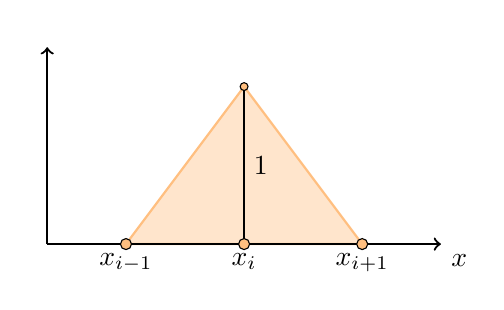
\begin{tikzpicture}[domain=0:4]
		%Triangle
		\draw [thick,-,orange!50!white, fill=orange!20!white] (1,0)--(2.5,2)--(4,0)--cycle;
		\draw[thick, -] (2.5, 0) -- (2.5,2);
		%Axis
		\draw[thick,->] (0,0) -- (5,0) node[below right] {$x$};
		\draw[thick,->] (0,0) -- (0,2.5) node[above left] {};
		%Points
		\draw[fill=orange!50!white, draw=black] (2.5,2) circle (0.5mm) node[above right]{};
		\draw[fill=orange!50!white, draw=black] (4,0) circle (0.7mm) node[below]{$x_{i+1}$};
		\draw[fill=orange!50!white, draw=black] (1,0) circle (0.7mm) node[below]{$x_{i-1}$};
		\draw[fill=orange!50!white, draw=black] (2.5,0) circle (0.7mm) node[below]{$x_i$};
		%Node
		\node[right] at (2.5,1) {$1$};
		\end{tikzpicture}
		\caption{Función $\phi_i(x)$}
		\label{fig:phi}
	\end{figure}
	
	Como base de nuestro espacio consideramos:
	\begin{equation*}
		\phi_i(x) =
		\left\{
		\begin{array}{l r}
			1-\left|\frac{x-x_i}{h}\right| & x\in[x_{i-1}, x_{i+1}]\\
			0 & x\notin[x_{i-1}, x_{i+1}]
		\end{array}
		\right.
		=
		\left\{
		\begin{array}{l r}
			\frac{x-x_{i-1}}{x_i-x_{i-1}} & x\in[x_{i-1}, x_i]\\
			\frac{x_{i+1}-x}{x_{i+1}-x_i} & x\in[x_{i}, x_{i+1}]\\
			0 & x\notin[x_{i-1}, x_{i+1}]
		\end{array}
		\right.
	\end{equation*}
    En la Figura \ref{fig:phi} se puede observar la forma de este tipo de funciones, que son claramente de $H_0^1(0,1)$.
	Tenemos por tanto que:
	\begin{equation*}
		\phi_i^\prime =
		\left\{
		\begin{array}{l l}
			\frac{1}{h} & x\in[x_{i-1}, x_i]\\
			\frac{-1}{h}  & x\in[x_{i}, x_{i+1}]\\
			0 & x\notin[x_{i-1}, x_{i+1}]
		\end{array}
		\right.
	\end{equation*}
	\paragraph{Cálculo de la forma bilineal}
	Dado que se tiene que los elementos $a_{ij}$ son nulos si $|i-j|>1$, tenemos que la matriz $A$ es tridiagonal. Tenemos que calcular:
	$$a(\phi_i, \phi_j) = \varepsilon\int_{0}^{1} \phi_i^\prime\phi_j^\prime + \int_{0}^{1}\phi_i^\prime\phi_j$$
	Para ello calculamos, para el primer término:
	\begin{itemize}
		\item $\int_{0}^{1} \phi_i'\phi_{i-1}' = \int_{x_{i-1}}^{x_i} -\frac{1}{h}\frac{1}{h} = h\cdot\frac{-1}{h^2} = \frac{-1}{h}$
		
		\item $\int_{0}^{1}(\phi_i')^2 = \int_{x_{i-1}}^{x_i}\left(\frac{1}{h}\right)^2 + \int_{x_i}^{x_{i+1}} \left(-\frac{1}{h}\right)^2 = \frac{2}{h}$
		
		\item $\int_0^1 \phi_i'\phi_{i+1}'=\int_{x_i}^{x_{i+1}}-\frac{1}{h}\frac{1}{h} = h\cdot\frac{-1}{h^2} = \frac{-1}{h}$
	\end{itemize}
	Y para el segundo:
	\begin{itemize}
		\item $\int_{0}^{1} \phi_i'\phi_{i-1} =
		\frac{1}{h}\int_{x_{i-1}}^{x_{i}}\phi_{i-1}  + \frac{-1}{h}\int_{x_{i}}^{x_{i+1}} \phi_{i-1} =
		\frac{1}{h}\frac{h}{2} = \frac{1}{2}$
		
		\item $\int_{0}^{1} \phi_i'\phi_{i} =
		\frac{1}{h}\int_{x_{i-1}}^{x_{i}}\phi_{i}  + \frac{-1}{h}\int_{x_{i}}^{x_{i+1}} \phi_{i}
		= \frac{1}{h}\frac{h}{2} + \frac{-1}{h}\frac{h}{2} = 0$
		
		\item $\int_{0}^{1} \phi_i'\phi_{i+1} =
		\frac{1}{h}\int_{x_{i-1}}^{x_{i}}\phi_{i+1}  + \frac{-1}{h}\int_{x_{i}}^{x_{i+1}} \phi_{i+1} =
		\frac{-1}{h}\frac{h}{2} = -\frac{1}{2}$
	\end{itemize}
	Tenemos por tanto que la matriz $A$ es de la forma:
	\begin{equation*}
		A = (a_{ij}) = 
		\left\{
		\begin{array}{l l l}
			\varepsilon \cdot {-1}/{h} + \frac{1}{2} & i = j-1 & \text{(Diagonal superior)}\\
			\varepsilon \cdot {2}/{h} & i = j & \text{(Diagonal principal)}\\
			\varepsilon \cdot {-1}/{h} - \frac{1}{2} & i = j+1 &  \text{(Diagonal inferior)}
		\end{array}
		\right.
	\end{equation*}
	\paragraph{Cálculo del operador lineal:}
	En este caso es sencillo calcular
	$$l(\phi_j) = \int_0^1 \phi_j = \frac{2h}{2} = h$$
	\paragraph{Resolución del sistema lineal:}
	Una vez que tenemos calculado la matriz $A$ y el vector $F$, sólo nos queda programar en \textsc{MatLab} una función que realice la aproximación resolviendo el sistema:
	$$AU = F$$
	\subsection{Programación del método}
	A continuación se muestra el código en \textsc{MatLab} de la aproximación a la solución utilizando elementos finitos a partir de un valor para $h$ y para $\varepsilon$:
	\lstset{style=matlabStyle}
	\lstinputlisting{../src/fem.m}
	\subsection{Análisis del error}
	En esta sección se realizará un estudio del error de las aproximaciones a la solución del problema utilizando distintos valores de $h$ y de $\varepsilon$. En las figuras \ref{fig:sfig1} y \ref{fig:sfig2} se pueden observar las distintas gráficas obtenidas para los valores:
	\begin{center}	
		\framebox{$h=$ 0.1, 0.05, 0.025, 0.0125} y \framebox{$\varepsilon=$ 0.1, 0.01, 0.005}
	\end{center}
	La formulación débil del problema que vimos en la sección anterior consiste en encontrar $u\in H_0^1(0,1)$ de tal forma que:
	$$a(u,v) = l(v)\ \forall v\in H_0^1(0,1)$$
	La aproximación por elementos finitos implica la búsqueda de $u_h\in V_h$, siendo $V_h$ un espacio finito dimensional de $H_0^1(0,1)$ de tal forma que:
	$$a(u_h, v_h) = l(v_h) \ \forall v_h\in V_h$$
	La formulación variacional es también válida para cualquier $v=v_h\in V_h$ siendo:
	$$a(u, v_h) = l(v_h)\ \forall v_h\in V_h$$
	Si restamos este resultado a la aproximación por elementos finitos, obtenemos:
	$$a(u-u_h, v_h) = 0\ \forall v_h\in V_h$$
	obteniendo la propiedad conocida como \textbf{ortogonalidad de Galerkin}.
	Con dicha propiedad y utilizando la coercividad de la forma bilineal con $v=u-u_h$ se tiene:
	$$||u-u_h||_{H^1(0,1)}^2\le \frac{1}{c_0}a(u-u_h, u-v_h)$$
	Ahora usamos la propiedad de continuidad y obtenemos:
	$$a(u-u_h, u-v_h)\le c_1||u-u_h||_{H^1(0,1)}||u-v_h||_{H^1(0,1)}$$
	Combinando ambos resultados obtenemos el lema de Céa:
	\begin{lemma}[Lema de Céa]
		La aproximación por elementos finitos $u_h$ es la mejor aproximación de $u\in H_0^1(\Omega)$ en $V_h$ salvo la constante $\frac{c_1}{c_0}$, es decir
		$$||u-u_h||_{H^1(\Omega)}\le \frac{c_1}{c_0}\min_{v_h\in V_h}||u-v_h||_{H^1(\Omega)}$$
	\end{lemma}
	El interpolador $\mathcal{I}_h u(x) = \sum_{i=1}^{N(h)-1} u(x_i)\phi_i(x)$ mejora si se refina la malla de elementos finitos. Luego tenemos que:
	$$\min_{v_h\in V_h} ||u-v_h||_{H^1(\Omega)} \le C(u)h^p$$
	Este resultado, combinado con el lema de Céa, produce una cota de error a priori:
	$$||u-u_h||_{H^1(\Omega)}\le C(u)\left(\frac{c_1}{c_0}\right)h^p$$
	Tenemos, por tanto, que un refinado del mallado hace que la aproximación por elementos finitos converja a la solución con la norma $H^1(\Omega)$.
	\newpage
	Dado que tenemos que $c_1=\varepsilon + C_{PF}$ y $c_0 = \varepsilon$. Si $\varepsilon << 1$ ocurre que la constante $\frac{c_1}{c_0} >> 1$. Se puede observar que se tiene una degradación de las aproximaciones cuando $\varepsilon << 1$, produciéndose grandes oscilaciones y teniendo que refinar mucho el mallado para que se produzca una reducción del error global (ver figuras \ref{fig:sfig1} y \ref{fig:sfig2}).
	\begin{center}
		\begin{figure}
			\makebox[\textwidth][c]{
				\begin{subfigure}{.7\textwidth}
					\centering
					\includegraphics[width=1\linewidth]{../img/1.png}
					\caption{$h = 0.1$, $\varepsilon =0.1 $}
					\label{fig:sfig11}
				\end{subfigure}%
				\begin{subfigure}{.7\textwidth}
					\centering
					\includegraphics[width=1\linewidth]{../img/4.png}
					\caption{$h = 0.05$, $\varepsilon =0.1 $}
					\label{fig:sfig14}
				\end{subfigure}%
			}
			
			\makebox[\textwidth][c]{
				\begin{subfigure}{.7\textwidth}
					\centering
					\includegraphics[width=\linewidth]{../img/2.png}
					\caption{$h = 0.1$, $\varepsilon =0.01 $}
					\label{fig:sfig12}
				\end{subfigure}%
				\begin{subfigure}{.7\textwidth}
					\centering
					\includegraphics[width=1\linewidth]{../img/5.png}
					\caption{$h = 0.05$, $\varepsilon =0.01 $}
					\label{fig:sfig15}
				\end{subfigure}%
			}
			
			\makebox[\textwidth][c]{
				\begin{subfigure}{.7\textwidth}
					\centering
					\includegraphics[width=1\linewidth]{../img/3.png}
					\caption{$h = 0.1$, $\varepsilon =0.005 $}
					\label{fig:sfig13}
				\end{subfigure}%
				\begin{subfigure}{.7\textwidth}
					\centering
					\includegraphics[width=1\linewidth]{../img/6.png}
					\caption{$h = 0.05$, $\varepsilon =0.005 $}
					\label{fig:sfig16}
				\end{subfigure}%
			}
			\caption{Aproximación con elementos finitos (I)}
			\label{fig:sfig1}
		\end{figure}
	\end{center}%
	\begin{center}
		\begin{figure}
			\makebox[\textwidth][c]{
				\begin{subfigure}{.7\textwidth}
					\centering
					\includegraphics[width=1\linewidth]{../img/7.png}
					\caption{$h = 0.025$, $\varepsilon = 0.1$}
					\label{fig:sfig21}
				\end{subfigure}%
				\begin{subfigure}{.7\textwidth}
					\centering
					\includegraphics[width=1\linewidth]{../img/10.png}
					\caption{$h = 0.0125$, $\varepsilon = 0.1$}
					\label{fig:sfig24}
				\end{subfigure}%
			}
			
			\makebox[\textwidth][c]{
				\begin{subfigure}{.7\textwidth}
					\centering
					\includegraphics[width=\linewidth]{../img/8.png}
					\caption{$h = 0.025$, $\varepsilon = 0.01$}
					\label{fig:sfig22}
				\end{subfigure}%
				\begin{subfigure}{.7\textwidth}
					\centering
					\includegraphics[width=1\linewidth]{../img/11.png}
					\caption{$h = 0.0125$, $\varepsilon = 0.01$}
					\label{fig:sfig25}
				\end{subfigure}%
			}
			
			\makebox[\textwidth][c]{
				\begin{subfigure}{.7\textwidth}
					\centering
					\includegraphics[width=1\linewidth]{../img/9.png}
					\caption{$h = 0.025$, $\varepsilon = 0.005$}
					\label{fig:sfig23}
				\end{subfigure}%
				\begin{subfigure}{.7\textwidth}
					\centering
					\includegraphics[width=1\linewidth]{../img/12.png}
					\caption{$h = 0.0125$, $\varepsilon = 0.005$}
					\label{fig:sfig26}
				\end{subfigure}%
			}
			\caption{Aproximación con elementos finitos (II)}
			\label{fig:sfig2}
		\end{figure}
	\end{center}
	\newpage
	\section{Error a posteriori}
	En este apartado se estudiará  el estimador a posteriori del error $||u-u_h||_{L_2(0,1)}$ para el problema propuesto.
	Nuestra ecuación es:
	$$-\varepsilon u'' + u' = 1$$
	Sabemos que para un problema como el siguiente:
	\begin{equation*}
	\left\{
	\begin{array}{l l}
	-u''+b(x)u'+c(x)u = f(x) & x\in(0,1)\\
	u(0) = u(1) = 0
	\end{array}
	\right.
	\end{equation*}
	se tiene el siguiente resultado:
	\begin{equation*}
		||u-u_h||_{L_2(0,1)} \le K_0\left(\sum_{i=1}^{N}h_i^4||R(u_h)||_{L_2(x_{i-1},x_i)}^2\right)^{1/2}
	\end{equation*}
	con la constante $K_0$ definida como sigue:
	$$K_0 = \frac{1}{\pi^2}\left(1+\frac{1}{\sqrt{2}}||b||_{L_\infty(0,1)}+\frac{1}{2}||c-b'||_{L_\infty(0,1)}\right)$$
	y el residuo de elementos finitos $R(u_h)$, con $x\in(x_{i-1}, x_i)$:
	$$R(u_h)(x) = f(x) + u_h^{\prime\prime}(x) -b(x)u_h^\prime(x)-c(x)u_h(x)$$
	Transformamos nuestra ecuación en la siguiente, multiplicándola por $1/\varepsilon$:
	$$-u'' + \frac{1}{\varepsilon}u' = \frac{1}{\varepsilon}$$
	De forma que tenemos:
	\begin{itemize}
		\item $b(x) = 1/\varepsilon$
		\item $c(x) = 0$
		\item $f(x) = 1/\varepsilon$
	\end{itemize}
	De esta forma:
	$$K_0 = \frac{1}{\pi^2}\left(1+\frac{1}{\varepsilon\sqrt{2}}\right)$$
	Por otro lado, como la aproximación $u_h$ es lineal a trozos, tenemos que su derivada segunda es nula, por tanto:
	$$R(u_h)(x) = \frac{1}{\varepsilon}\left(1-u_h'(x)\right)$$
	Luego, dado que $u_h(0) = u_h(1) = 0$:
	\begin{align*}
	\sum_{i=1}^N||R(u_h)(x)||_{L_2(x_{i-1},x_i)}^2 &= \frac{1}{\varepsilon^2}\sum_{i=1}^{N} \int_{x_{i-1}}^{x_i}(1-u_h')^2\\
	&=  \frac{1}{\varepsilon^2} \int_{0}^{1}1+(u_h')^2 - 2u_h'\\
	& = \frac{1}{\varepsilon^2} + \frac{1}{\varepsilon^2} \int_{0}^{1}(u_h')^2 - \int_0^1 2u_h'\\
	& = \frac{1}{\varepsilon^2} + \frac{1}{\varepsilon^2} \int_{0}^{1}(u_h')^2 \left.-2u_h\right|_0^1\\
	& = \frac{1}{\varepsilon^2} + \frac{1}{\varepsilon^2} \int_{0}^{1}(u_h')^2\\
	&= \frac{1}{\varepsilon^2}\left(1+\int_0^1 (u'_h)^2\right)
	\end{align*}
	La integral del término derecho se calcula como sigue:
	$$\int_0^1 (u_h')^2 = \int_0^1 \left(\sum_{i=1}^{N-1}u_h(x_i)\phi_i'\right)\left(\sum_{j=1}^{N-1}u_h(x_j)\phi_j'\right)$$
	Matricialmente:
	\begin{equation*}
		\int_0^1 (u_h')^2 =
		\left[
			u_h(x_1) \hdots  u_h(x_{N-1})
		\right]
		\begin{bmatrix}
			2/h  & -1/h & \hdots & 0\\
			-1/h &  2/h & \ddots & \vdots\\
			\vdots & \ddots & \ddots & -1/h\\
			0 & \hdots & -1/h & 2/h\\
		\end{bmatrix}
		\begin{bmatrix}
			u_h(x_1) \\ \vdots \\ \vdots \\ u_h(x_{N-1})
		\end{bmatrix}
	\end{equation*}
	Aunque no es necesario, se utilizará un mallado equiespaciado por cuestiones de simplicidad, luego tenemos:
	\begin{equation*}
		||u-u_h||_{L_2(0,1)} \le 
		\frac{h^2}{\pi^2}\left(1+\frac{1}{\varepsilon\sqrt{2}}\right)
		\left(\sum_{i=1}^{N}||R(u_h)||_{L_2(x_{i-1},x_i)}^2\right)^{1/2}
	\end{equation*}
	\newpage
	\subsection{Programación en \textsc{MatLab}}
	A continuación se muestra el código realizado en \textsc{MatLab} del estimador a posteriori:
		\lstset{style=matlabStyle}
		\lstinputlisting{../src/post_bound.m}
	Tras la programación en \textsc{MatLab}, se ha obtenido la cota del error para los valores 
	\begin{center}	
		\framebox{$h=$ 0.1, 0.05, 0.025, 0.0125, 0.01, 0.005} y \framebox{$\varepsilon=$ 0.1}
	\end{center}
	En la Figura \ref{fig:p1} se puede observar el resultado del estimador en función del tamaño del mallado $h$ (en escala logarítmica). Se ha obtenido una pendiente de $2$, es decir, el error global estimado es de orden 2 con respecto al tamaño del mallado. Para obtener la pendiente de la recta representada se ha utilizado la siguiente función de \textsc{MatLab}:
	\begin{lstlisting}
		% h: vector of mesh sizes.
		% B: vector of bounds.
		poly = polyfit(log(h), log(B) , 1);
		slope = poly(1)
	\end{lstlisting}
	
	\newpage
	Además de esto, se han representado, también en escala logarítmica, los errores estimados y los errores reales descritos en la siguiente tabla, correspondiente a $\varepsilon = 1$:
	\begin{center}
		\begin{tabular}{|c|c|}
			\hline
			\rowcolor[HTML]{EFEFEF} 
			\textbf{$n=1/h$} & \textbf{$||u-u_h||_{L_2(0,1)}$} \\ \hline
			$10$             & $0.0151$                        \\ \hline
			$20$             & $0.0039$                        \\ \hline
			$40$             & $9.7229\cdot 10^{-4}$           \\ \hline
			$80$             & $2.4342\cdot 10^{-4}$           \\ \hline
		\end{tabular}
	\end{center}
	En la gráfica de la Figura \ref{fig:p2} se puede observar que ambas rectas tienen la misma pendiente y la recta del error estimado queda siempre por encima de la de errores reales, pues representa una cota de estos últimos.
	\begin{center}
		\begin{figure}[h]
			\makebox[\textwidth][c]{
				\begin{subfigure}{.7\textwidth}
					\centering
					\includegraphics[width=1\linewidth]{../img/post_h.png}
					\caption{$h$ frente al error en escala logarítima.}
					\label{fig:p1}
				\end{subfigure}%
				\begin{subfigure}{.7\textwidth}
					\centering
					\includegraphics[width=1\linewidth]{../img/post_N.png}
					\caption{$N$ frente al error en escala logarítima.}
					\label{fig:p2}
				\end{subfigure}%
			}
			\caption{Estimador del error a posteriori}
			\label{fig:p0}
		\end{figure}
	\end{center}
\end{document}